\chapter{Estructura de datos de los documentos CEA}
\section*{Características Generales}

Ambos documentos corresponden a una solicitud generada a partir de la creación de un proyecto que determina cierta información que será necesaria recopilar bajo distintas metodologías.

El documento FL33 corresponde a una solicitud de servicio interna desde algún área en particular del CEA hacia el laboratorio de química, con el fin de obtener distintos estudios de parámetros químicos y solicitar materiales y equipos para la obtención de estos.

El documento R08 corresponde a una solicitud de compra que se entrega de manera interna al Área de Finanzas que gestionará adecuadamente la solicitud para obtener la autorización y realizar la compra.

En cuanto a los formatos de cada documento, estos se diferencian en que FL33 es un documento de texto (por ejemplo: word) y el R08 es una tabla de planilla de cálculo (por ejemplo: excel).

Ahora bien, se presentan ciertas similitudes en cuanto a la información que tiene cada uno, principalmente acerca del proyecto y quien es el responsable de la solicitud.

También tienen diferencias importantes, en uno se concentra la información en la solicitud del análisis químico de cada parámetro correspondiente a cada matriz, en otro se concentra mayormente en el aspecto de los costos que tiene cada análisis según la información entregada por cada laboratorio externo. 

\begin{figure}
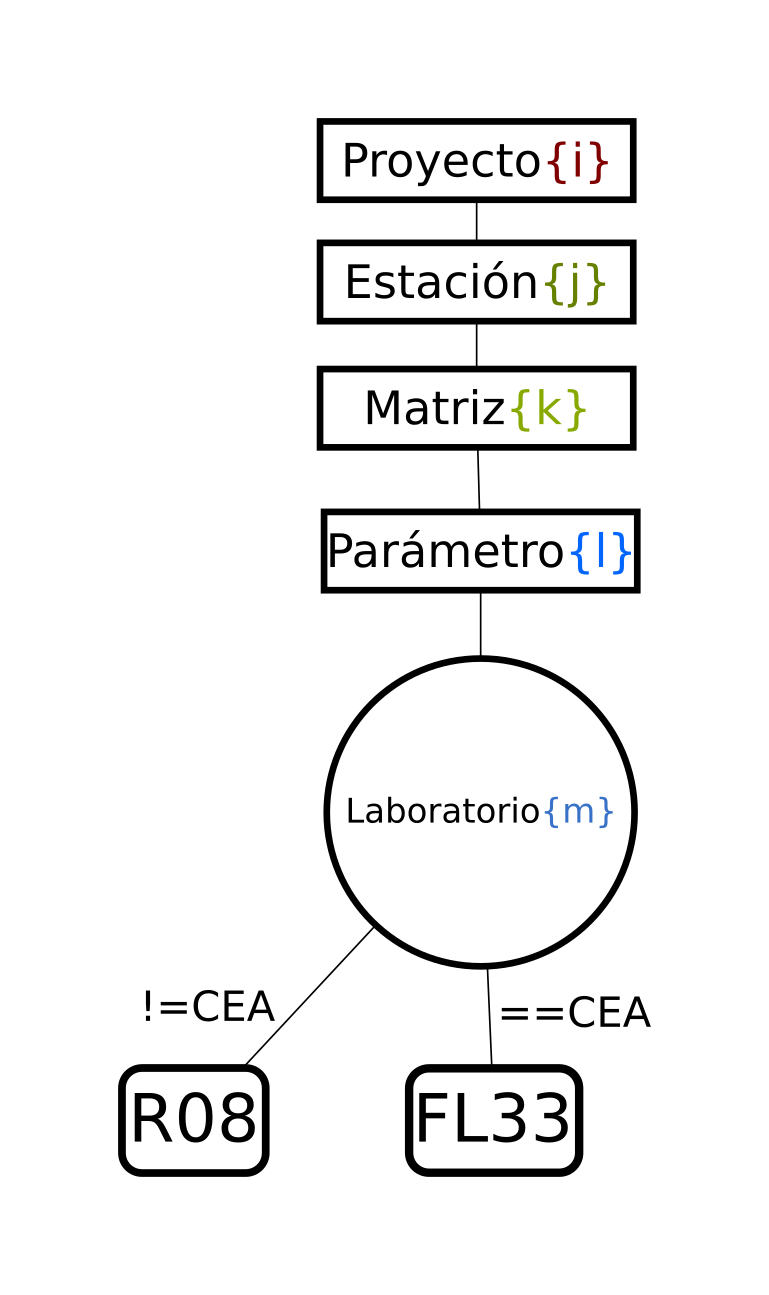
\includegraphics[scale=.8]{estruc_general.png}
\caption{Determinación del Documento a Generar}
\label{determinacion_doc}
\end{figure}

Hay, además, dos aspectos a considerar en la caracterización de cada documento

\begin{itemize}
	\item Plantilla o estrucura de presentación
	\item Secciones de información
\end{itemize}

\section*{Características Particulares}

En esta sección se estudiarán las características particulares que nos permitirán definir las agrupaciones de información adecuadas para generar el proceso de automatización.

\subsection*{FL33: Solicitud de Servicio}

Puedes obtenerlo de este enlace: \href{https://www.mediafire.com/?9e5cemqvsqo31a4}{Descarga FL33}

\subsubsection{Plantilla}

Tiene un encabezado estandar que aparece en todas las páginas del documento, a la izquierda contiene el logo de CEA laboratorio, al medio nombre de documento, a la derecha la identificación en codigo y el número asignado. Figura \ref{encabezado_fl33}.

\begin{figure}
	\centering
	
\includegraphics[scale=.7]{fl33_encabezado.png}
	\caption{Encabezado del FL33}
	\label{encabezado_fl33}
\end{figure}

En el cuerpo de texto contiene, en la primera página los antecedentes de proyecto, desde la primera los antecedentes analíticos y en la última la solicitud de materiales y equipos. Figura \ref{cuerpo_fl33}.

\begin{figure}
	\centering
	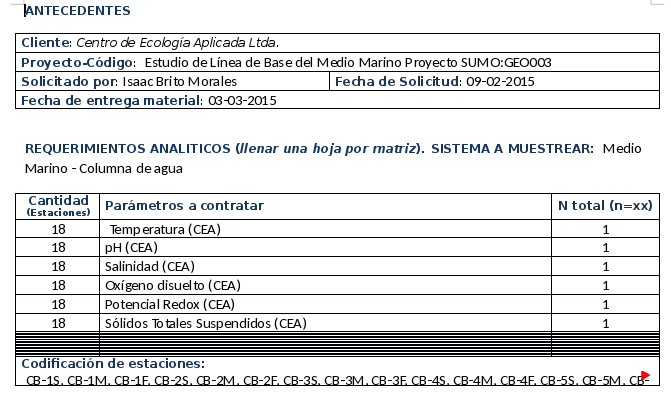
\includegraphics[scale=.7]{fl33_cuerpo.png}
	\caption{Cuerpo del FL33}
	\label{cuerpo_fl33}
\end{figure}

En el pie de página contiene indicaciones de requerimientos, información de número de página y datos de versión (número y fecha). Figura \ref{footer_fl33}.

\begin{figure}
	\centering
	
\includegraphics[scale=.7]{fl33_footer.png}
	\caption{Pie de página del FL33}
	\label{footer_fl33}
\end{figure}

\subsubsection{Secciones}

Consiste en tres secciones en las que será necesario ingresar la información. Tradicionalmente es de forma manual pero esto cambia con la implementación de la solución que trata este documento.

La primera sección corresponde a la información general del proyecto, se llama \textit{Antecedentes}. Figura \ref{antecedentes_fl33}. Se compone de los siguientes ítems:

\begin{itemize}
	\item Nombre del Cliente
	\item Proyecto y Código
	\item Quien solicita el servicio
	\item Fecha de Solicitud
	\item Fecha entrega de Material
\end{itemize}

\begin{figure}
	\centering
	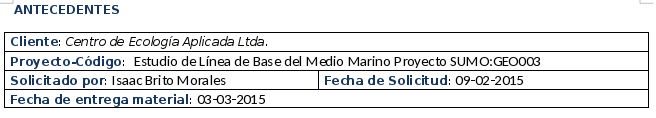
\includegraphics[scale=.7]{fl33_antecedentes.png}
	\caption{Tabla de Antecedentes del FL33}
	\label{antecedentes_fl33}
\end{figure}

La siguiente sección comprende la información listada de cada parámetro a medir. Comprende una tabla (ver figura \ref{matriz_fl33}) que permite detallar la siguiente información:

\begin{itemize}
\item Cantidad de Estaciones
\item Parámetro 
\item Réplicas por parámetro
\item Lista de estaciones
\item Observaciones
\end{itemize}

\begin{figure}
	\centering
	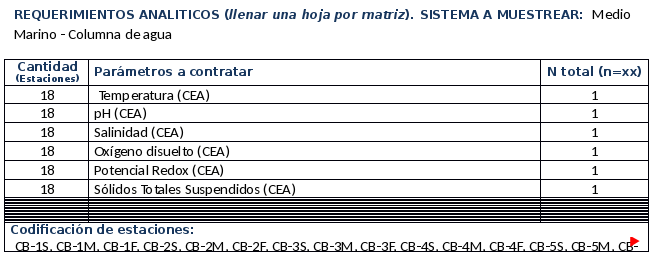
\includegraphics[scale=.7]{fl33_matriz.png}
	\caption{Sección de parámetros por matriz en FL33}
	\label{matriz_fl33}
\end{figure}

Luego, la última sección corresponde al listado de materiales y equipos solicitados para la obtención de las muestras (ver figura \ref{equipos_fl33}).

\begin{figure}
	\centering
	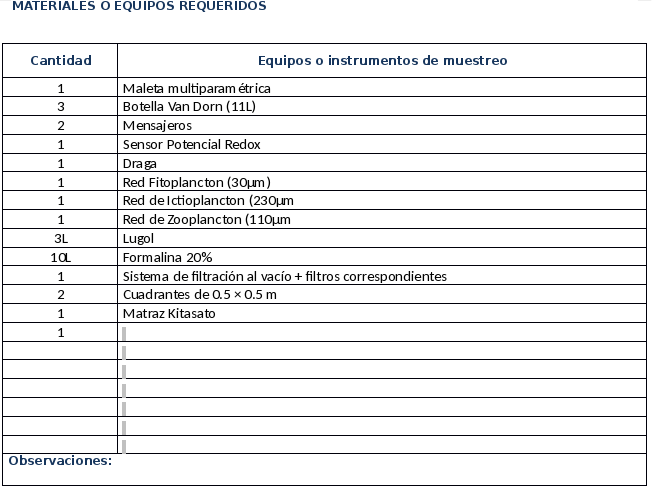
\includegraphics[scale=.7]{fl33_equipamiento.png}
	\caption{Sección de materiales y equipos por matriz en FL33}
	\label{equipos_fl33}
\end{figure}

\subsection*{R08: Orden de Compra}

Puedes obtenerlo de este enlace: \href{https://www.mediafire.com/?zgg9tstpdfm6fqi}{Descarga R08}

\subsubsection{Plantilla}

Es una planilla de cálculo adaptada a un formato de documento para contener la información de la orden de compra, contiene cuatro secciones generales en las que se ingresa la información.

\begin{itemize}
	\item Encabezado: es información sobre la clase de documento e identificadores institucionales.
	\item Información general: es información sobre el proyecto y fechas de compra.
	\item Detalle de compras: listado de elementos para las compras.
	\item Observaciones: comentarios en particular.
\end{itemize}

\subsubsection{Secciones}

La primera sección de informacón requiere completar los datos generales correspondientes a la solicitud (ver figura \ref{general_r08}), estos son 

\begin{itemize}
	\item Quien solicita la compra
	\item Fecha de solicitud
	\item Fecha de necesidad
	\item Código de proyecto asociado
	\item Nombre de empresa e información de contacto
	\item Área solicitante
	\item Si se adjunta algún documento
\end{itemize}

\begin{figure}
	\centering
	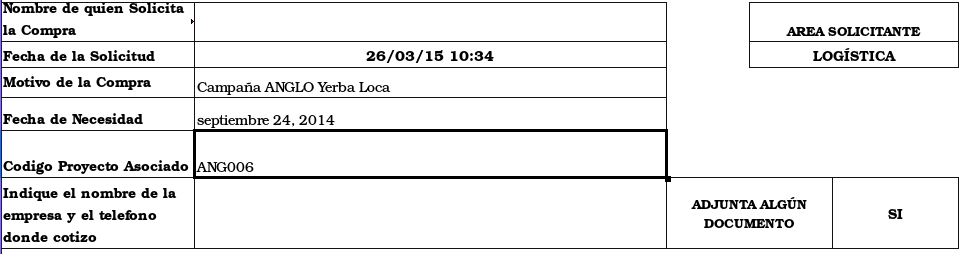
\includegraphics[scale=.5]{r08_general.png}
	\caption{Sección de información general R08}
	\label{general_r08}
\end{figure}

La siguiente sección corresponde al detalle de los elementos a comprar a la empresa en particular (ver figura \ref{detalle_r08}). Esta sección solicita los siguientes campos:

\begin{itemize}
	\item Cantidad de elementos
	\item Elemento
	\item Unidad de medida
	\item Valor unitario
	\item Valor neto total
	\item Moneda
\end{itemize}

\begin{figure}
	\centering
	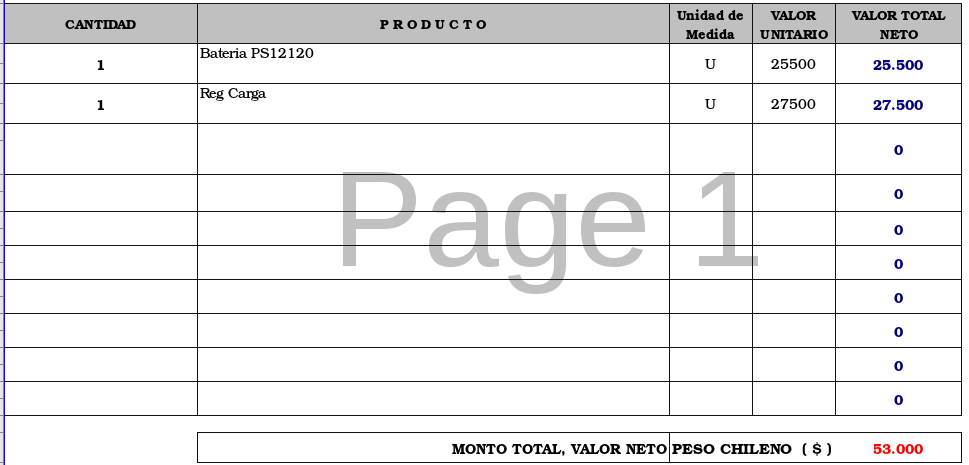
\includegraphics[scale=.5]{r08_detalle.png}
	\caption{Sección de información general R08}
	\label{detalle_r08}
\end{figure}

La última sección corresponde a las observaciones particulares sobre la solicitud de compra.

\section*{Agrupación de la Información}

Una vez analizados los documentos de llegada será necesario generar la abstracción de la información para determinar los grupos adecuados de categorias para poder realizar las funciones de transferencia desde la plantilla base a cada documento. 

\subsection{Abstracción para FL33}

Tal como se observa en figura \ref{determinacion_doc} se determina la generación de cada documento dependiendo en primer lugar del laboratorio, siendo para el documento FL33 correspondiente al laboratorio CEA. Por lo que es lógico partir agrupando desde el laboratorio que define el documento.

Luego, la sección de datos generales permite una agrupación, la sección de parámetros se determina mediante agrupaciones por matrices, la sección de equipos permite una agrupación.
En conjunto se puede definir una estrucura de datos como se observa en la figura \ref{estructura_datos_fl33}

\begin{figure}
	\centering
	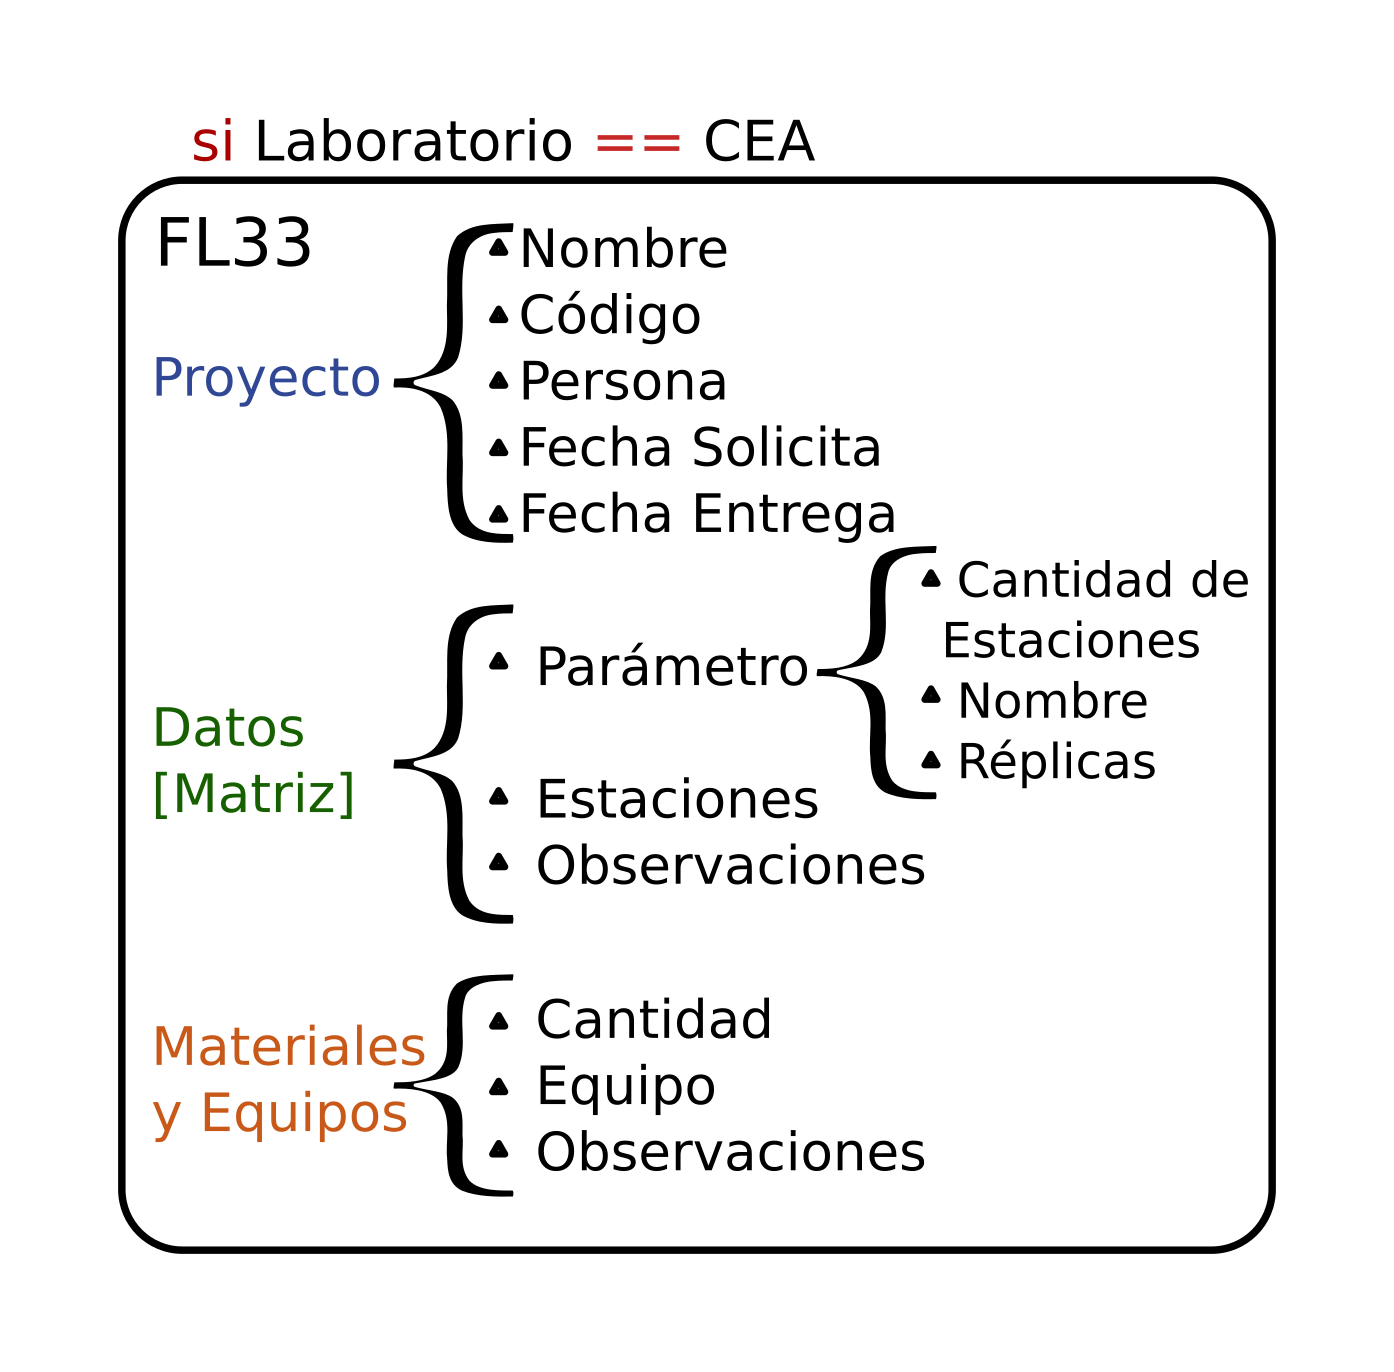
\includegraphics[scale=.7]{estructura_datos_fl33.png}
	\caption{Estructura de datos para FL33}
	\label{estructura_datos_fl33}
\end{figure}

\subsection{Abstracción para R08}

Nuevamente, según la  figura \ref{determinacion_doc}, las ordenes de compra se generan para cualquier laboratorio externo (distinto a CEA). El enfoque de este documento radica en las cantidades y valores de cada producto (elemento) cotizado.

Según las secciones observadas, la primera permite agrupar datos de proyecto y de solicitud, la segunda agrupa a los productos, cantidades y precios, la tercera agrupa las observaciones. En conjunto se puede definir una estrucuta de datos como se observa en la figura \ref{antecedentes_r08}


\begin{figure}
	\centering
	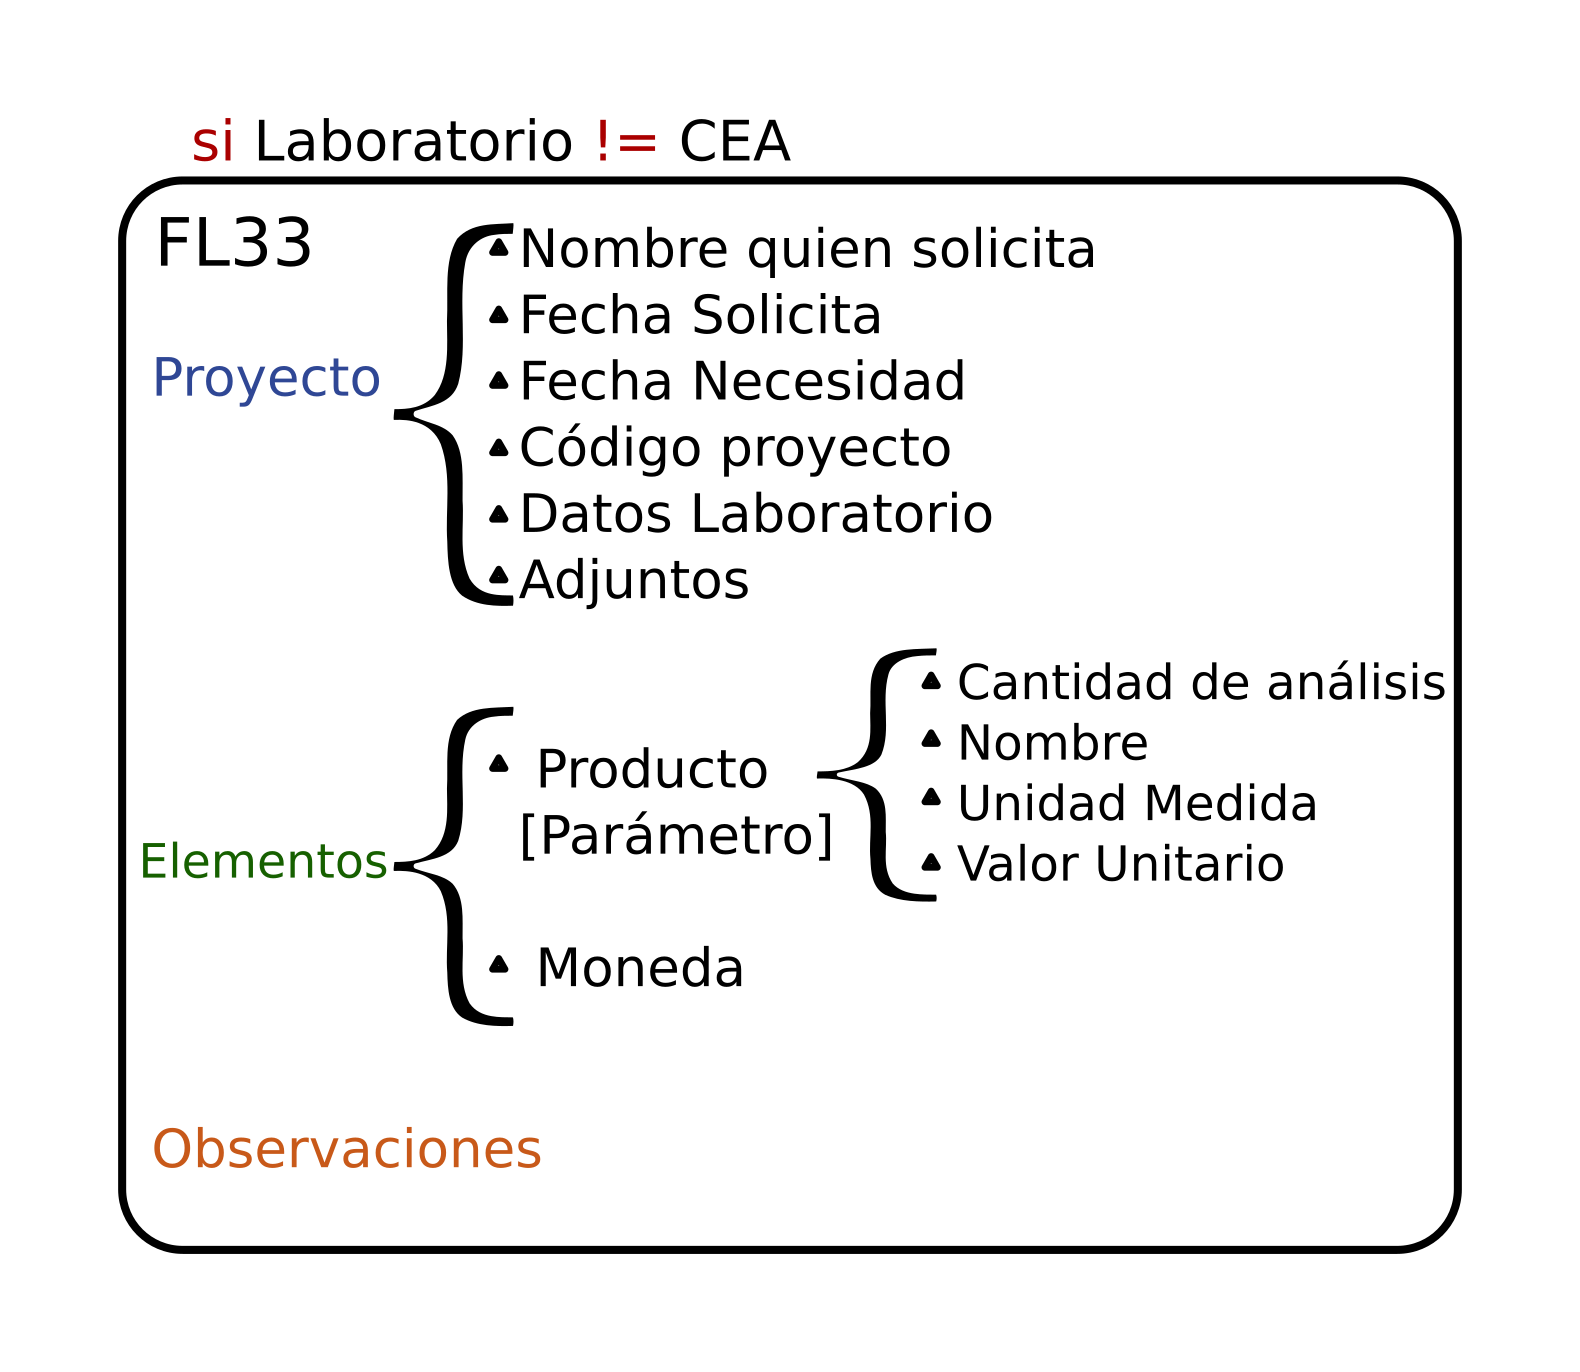
\includegraphics[scale=.6]{estructura_datos_r08.png}
	\caption{Estructura de datos para R08}
	\label{estructura_datos_r08}
\end{figure}

